\ofsection{Players}
%
\ofquote{"I am THE Basch fon Ronsenburg!"\\}{Vaan}\\\\
%
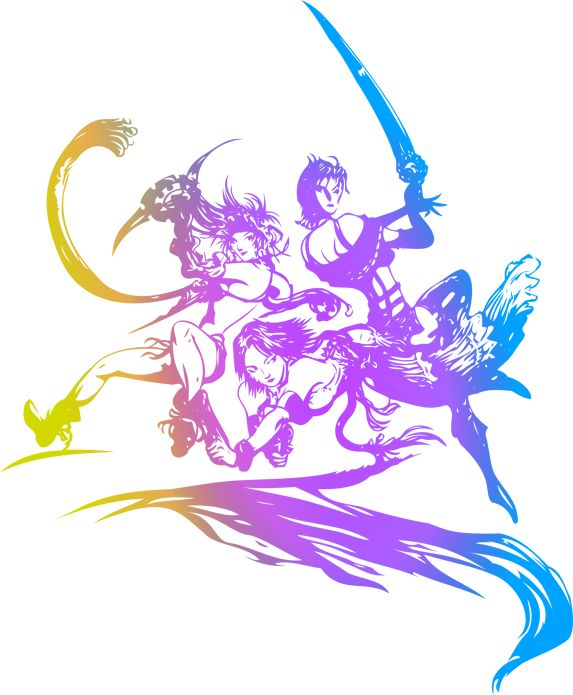
\includegraphics[width=\columnwidth]{./art/images/ff10-2.jpg}
%
\vfill
%
Every player creates a \accf{Character} who is a protagonist in the game world created by the GM.
To create a Level~1 character, copy or print the \accf{Character Sheet} on the next page.
It allows you track various aspects about your character and there is an example of a filled out sheet, that you can use as a guideline.
Choose your character's \accf{Name} and give a short description of him or her.
Briefly summarize your character's \accf{Story} and explain his or her motivation for joining the party, considering that this is most likely his or her first serious adventure.
Then choose a \accf{Job} for your character as explained below. 
Finally, the \accf{Equipment} subsection explains how you can customize your character's starting equipment.
The table on the right summarizes the benefits gained at further Levels, all of which are explained in detail within this section.
%
\vfill
%
Your character's \accf{Job} determines his or her combat proficiency including abilities, attributes and equipment expertise.
All available Jobs are detailed in their Job descriptions right after the character sheets.
Print or copy the description of your chosen Job to use as the second page of your character sheet.
Your character's attributes are initially 0 and increase by progressing in a job.
The job description shows the attributes and abilities gained at each Level as well as the types of equipment your character can use.
When your character reaches Level~3, you have to decide between one of the job's two \accf{Archetypes}. 
Archetypes represent different specializations of a Job and provide additional abilities and attributes.
%
\newpage
%
\ofboxwithtitle{Example: Character Creation}
{
	We create a character named Vaan, who is a 17-year old, blonde human boy with athletic appearance. 
	Vaan is an orphan, who gets by in the big city by stealing and often acts as a father figure to other orphans.
	He dreams of owning an airship and being a sky pirate one day.
	From the attributes table of the job we determine Vaan's maximum HP~(20), maximum MP~(19) and AGI (4), all other attributes start at 0.
	We also note that he learns the Steal tech.
	Finally, from our initial 1500G, we buy a Mythril Knife, Myhtril Vest, a Phoenix Down and 2 Potions, which leaves us with 300G extra.
}
%
\vfill
%
\oftable{p{0.3\columnwidth} p{0.7\columnwidth}}
{\accf{Level} & \accf{Benefit Gained}}
{
	1 & Job, Beginner Equipment \ofrow
	2 & Talent \ofrow
	3 & Archetype \ofrow
	4 & Limit Break, Advanced Equipment \ofrow
	5 & Esper \ofrow
	6 & Specialization \ofrow
	7 & Specialization \ofrow
	8 & Specialization, Expert Equipment \ofrow
	9 & Specialization \ofrow
	10 & Specialization
}
%
\vfill
%
At Levels marked as \accf{Specialization}, you can chose from one of the following benefits that you character gains.
You cannot pick the same benefit more than once.\ofrow
\ofbullet{At the start of each session, add an additional 6 to the pool of Fortune Dice.}
\ofbullet{You gain a second Esper of your choice.}
\ofbullet{You gain a second Talent of your choice.}
\ofbullet{You gain a second Limit Mode, allowing you to acquire Limit Points from 2 sources. Also, the maximum Rating of your Limit Break is increased by 2.}
\ofbullet{You gain access to the second Archetype your job. You can switch between the two whenever you go to sleep and your attributes and abilities change depending on your currently active Archetype.}
\ofbullet{When you use a Spell, Tech or Reaction ability from your Archetype, its MP cost is halved and you gain 1 Limit Point.}
\ofbullet{All weapons and armor gain an additional Materia Slot as long as your have them equipped.} 
\ofbullet{You gain the ability to equip one additional weapon or armor type of your choice.} 
\ofbullet{Choose 4 from the following list of attribute bonuses. You cannot pick the same one more than twice:\newline HP+5, MP+5, STR+1, DEF+1, MAG+1, RES+1.}
%
\clearpage
%
\ofcs{}
%
\ofcs{
	name=Lightning,
	%
	description={%
		\vspace*{-0.5cm}
		\begin{multicols}{2}
			Age: 21\\Race: human\\Hair: rose\\Height: 1.70m\\Right-Handed\\ Determined\\ Cold
			\columnbreak\vspace*{-1.7cm}\\
			\hspace*{-1cm}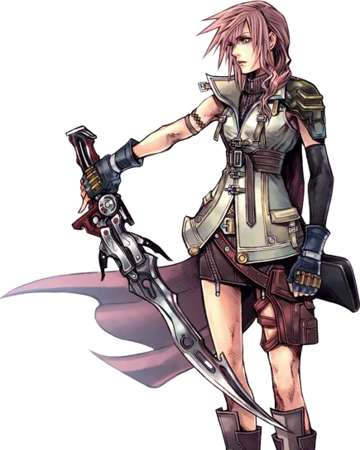
\includegraphics[width=1\columnwidth]{./art/charactersheets/claire.jpg}
		\end{multicols}
		\vspace*{-0.9cm}
	},
	%
	story={\\
		Both of my parents died when I was young. 
		I raised my sister Serah and joined the army where I became a sergeant. 
		But now Serah is in danger so I have quit the army to find her. \\\\\\
		"It's not a question of can or can't.\\ There are some things in life you just do."
	},
	% 
	hpcur=19, hpmax=91, mpcur=13, mpmax=85, agi=3, movement=4u, evasiondc=9, str=5, def=3, mag=7, res=2, 
	%
	level=8, job=Red Mage, archetype=Ravager\phantom{1234567}, talent=Guardian Corps,
	%
	abilities={Cure, Fire, Blizzard, Thunder, Blind,\\ Poison, Esuna, NulElement},
	specials={Overwhelm, Swiftcast}, status={Blind (1r), EnDEF (2r)},
	%
	limitbreak=Thundara, limitmode=Brave, limitpoints=\ofcslimitbarfilled, 
	limitdesc={A barrage of lightning strikes descends upon an enemy within 5u and everyone within 2u of him. All affect targets suffer 2d+8 lightning damage.},
	%
	summon=Odin, summonused=yes, summonsupport={Perform a short ritual to summon Odin's horse, Sleipnir.\\}, summonability={A target on the battlefield suffers KO on failed DC~8 check or damage equal to 3 times Level otherwise.},
	%
	weapon=Foldable Gunblade, weaponbox=\ofcsweaponboxexpert, weaponeffect=Ranged attack after ability, weapontype=counter on 11 or 12 enemy evasion check, armor=Guardian Corps Uniform, armorbox=\ofcsarmorboxbeginner, armortype=DEF~+1, accessory1=Power Armlet, accessory1effect=STR~+1,
	%
	gil=2009, inventory={\\Survival Knife, 5x Bomb Fragment, 5x Hi-Potion\\ 3x Remedy, 2x Phoenix Down, 1x Elixir}
}
%
\clearpage